% intro prargraph %

the best theoretical model we currently have that describes all the known fundamental particles and their interactions is known as the standard model theory 
%The standard model (SM) of particle physics is the best theoretical model we currently have that describes all the known fundamental particles and their interactions.

This chapter will reviews the basics of the SM theory .. (update when the content of chapter is compelet)

%..........................
%\section{The Standrad model}

Particles in the SM can be classified into two categories ,as shown in Fig.~\ref{fig:SMParticles}, based on their spin or Intrinsic Angular Momentum value: fermions have half integer spin, bosons have full integer spin.

Fermions particles include particles that make up matter this: electrons, protons and neutrons. All fermions follow Pauli exclusion principle which is essential for building atoms and the periodic table. This group of particles can be divided further more into two groups based on the strong force: leptons, do not have strong interactions, and quarks, have strong nuclear interactions.

Quarks cannot be isolated because of the color confinement. They are always found in a bound state known as hadrons interacting via strong force. Hadrons either composed of three quarks, baryons, or a pair of a quark and anti-quark, mesons. Baryons have half integer spin so they are considered fermions while mesons have integer spin so they are considered bosons.

Leptons group consist of three electrically charged particles (electron, muons, tau) and 3 electrically neutral neutrinos that comes in three flavors associated with the electron, muon, tau. The electrically charged leptons interact with all forces except for the strong force while Neutrinos only interact through gravity and weak force.

Each group in quarks  and leptons can be organized into three generations that only differ in their mass. The heavier generation can decay into the next lighter generation till we reach the lightest one that is stable like (electron, up and  down quarks). “Here insert table that shows these generations”

The force carry particles in the SM are vector bosons with spin 1. The electromagnetic force carried by the photon. The strong force is carried by 8 types of gluons. The weak interaction is carried by two charged W bosons and one neutral Z boson. Higgs boson is a scalar boson with spin 0 that interact with mass. as shown in Fig.~\ref{fig:SMinteractions}

(check if sm details are missing from draft1, also add figures)
% include anti matter and how is it associated with matter particles check J.notes purple highlight) 
% use the SM figure
% maybe breifly mention the sectors of SM this is : QCS, EW , strong 
%(consider adding the shortcoming of the SM and how those reasons motivatin the directon of the HEP)
% why SM is incomplete? gravit? 
%..........................     

\begin{figure}[t!]

\centering
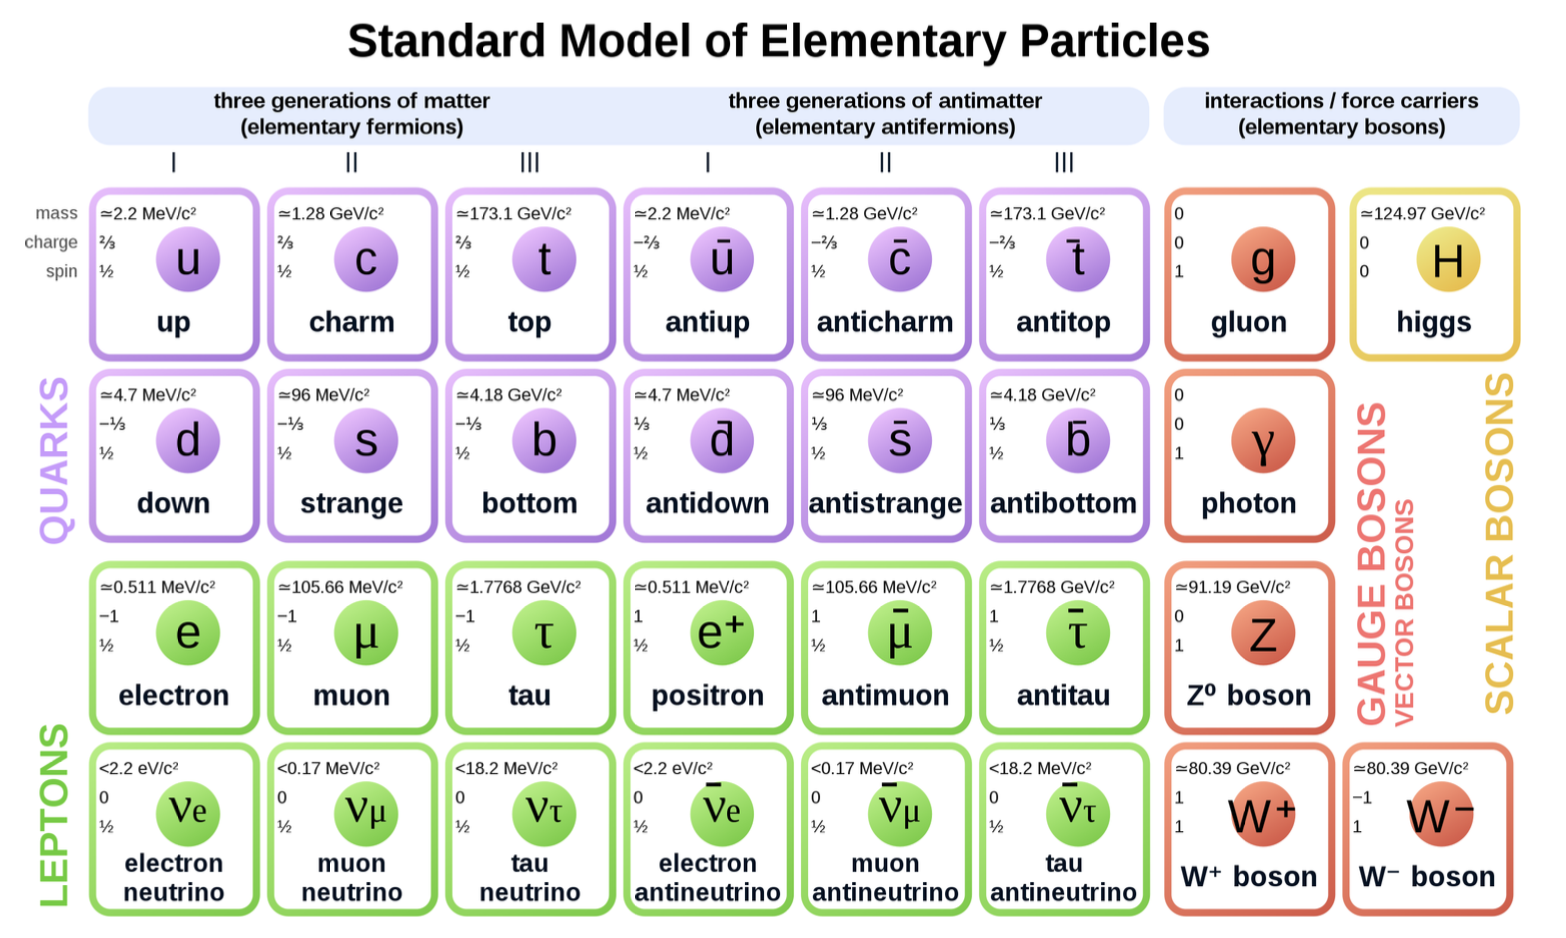
\includegraphics[width=0.99\textwidth]{figures/SM_include_antimatter.png}}
\caption[Summary of standard model fundamental particles]{Summary of SM fundamental particles. Figure source~\cite{SMtable}.
\label{fig:SMParticles}}

\end{figure}

\begin{figure}[t!]
\centering
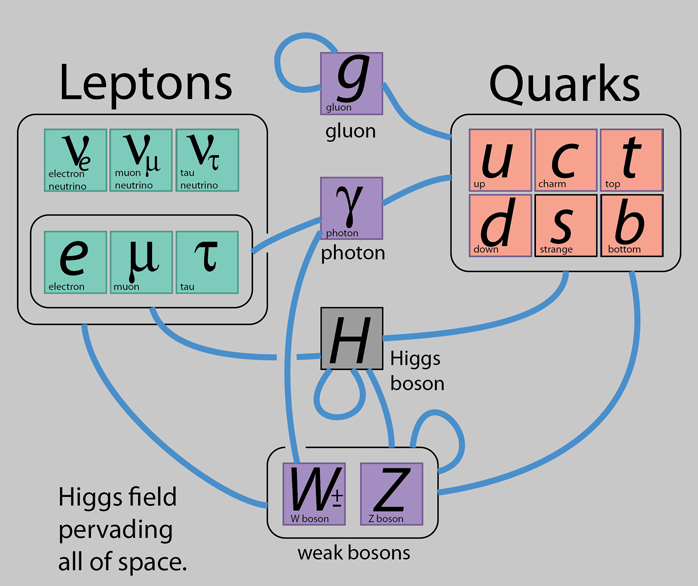
\includegraphics[width=0.99\textwidth]{figures/interactions_SM.png}}
\caption[Summary of standard model fundamental particles]{Summary of SM fundamental particles. Figure source~\cite{SMintera}.
\label{fig:SMinteractions}}
\end{figure} 
